\documentclass{article}
\usepackage{graphicx}
\usepackage{lmodern}
\usepackage[T1]{fontenc}
\usepackage{tabularx}
\usepackage{enumitem}
\usepackage{placeins}

\author{\large{Lorenzo Ricci}}
\title{\textbf{\fontsize{34pt}{45pt}\selectfont Dual Perceptron (dual form)}}
\date{}
\renewcommand*\contentsname{Sommario}

\begin{document}
	\begin{figure}
		\centering
		
\includegraphics[width=0.7\linewidth]{Unifi_nuovo.svg.png}
		\label{fig:unifinuovo}
	\end{figure}
	\maketitle
	\vspace*{2cm}
	\begin{center}
		\Large Università degli studi di Firenze\\ Corso di Laurea in Ingegneria Informatica\\ Intelligenza Artificiale\\ A.S. 22/23
	\end{center}
	\tableofcontents \newpage
    \section{Introduzione algoritmo}
    Il primo algoritmo iterativo per l'apprendimento di classificazioni lineari è la procedura proposta da Frank Rosenblatt nel 1956 per il perceptron. E' una procedura \textit{on-line} e \textit{mistake-driven},
    che inizia con un vettore peso iniziale \textbf{w0} (solitamente inizializzato tutto a 0, \textbf{w0=0}) e si adatta ogni volta che un punto, che sta venendo addestrato, viene malclassificato dai pesi attuali.
    L'algoritmo aggiorna il vettore peso e il bias direttamente. Inoltre questa procedura ha garantita la convergenza dall'esistenza di un iperpiano che classifica correttamente i punti su cui lo si sta facendo addestrare, e in questo
    caso si dice che i dati sono \textit{linearmente separabili}. Quindi, viceversa, se non esiste un iperpiano i dati si dicono non separabili. Si definisce \textit{margine funzionale di un esempio} ({$\textbf{x}_i$},$y_i$) con rispetto all'iperpiano (\textbf{w},b), la quantità:
    \begin{center}
        $\gamma_i$ = $y_i$(⟨$x_i$, $x_j$⟩+$b$) 
    \end{center}
    e si nota che se $\gamma$ > 0 implica una corretta classificazione di ({$\textbf{x}_i$},$y_i$).
    L'algoritmo Perceptron lavora quindi, aggiungendo esempi di addestramento positivi classificati in modo errato o sottraendo quelli negarivi classificati in modo errato ad un vettore peso scelto all'inizio in modo aribitrario.
    Senza perdita di generalità, se si assume che il vettore peso iniziale è un vettore zero, e che l'ipotesi finale sarà quella di essere una combinazione lineare dei punti di addestramento, possiamo ridefinire il vettore peso: 
    \begin{center}
        $\textbf{w}$ = $\displaystyle\sum_{i=1}^l \alpha_iy_i\textbf{x}_i$
    \end{center}
    dove, dal momento in cui il segno del coefficiente di $\textbf{x}_i$ è dato dalla classificazione di $y_i$, gli $\alpha_i$ sono volori positivi proporzionali al numero di volte in cui una classificazione errata di $\textbf{x}_i$ ha causato l'aggiornamento del peso.
    Punti che hanno causato pochi errori avranno un valore più piccolo di $\alpha_i$, viceversa punti più difficili avranno questo valore più grande.
    Quindi fissato un set di addestramento S, si può pensare al vettore \textbf{$\alpha$} come rappresentazione alternativa dell'ipotesi in coordinate diverse o duali.
    \newpage
    \section{Implementazione} 
    Lo scopo del seguente progetto è quello di implementare l'algoritmo nella sua forma duale descritto in (Cristianini \& Shawe-Taylor 1999), permettendo l'uso di funzioni kernel al posto del prodotto
    scalare ⟨xi, xj⟩.
    \begin{center}
        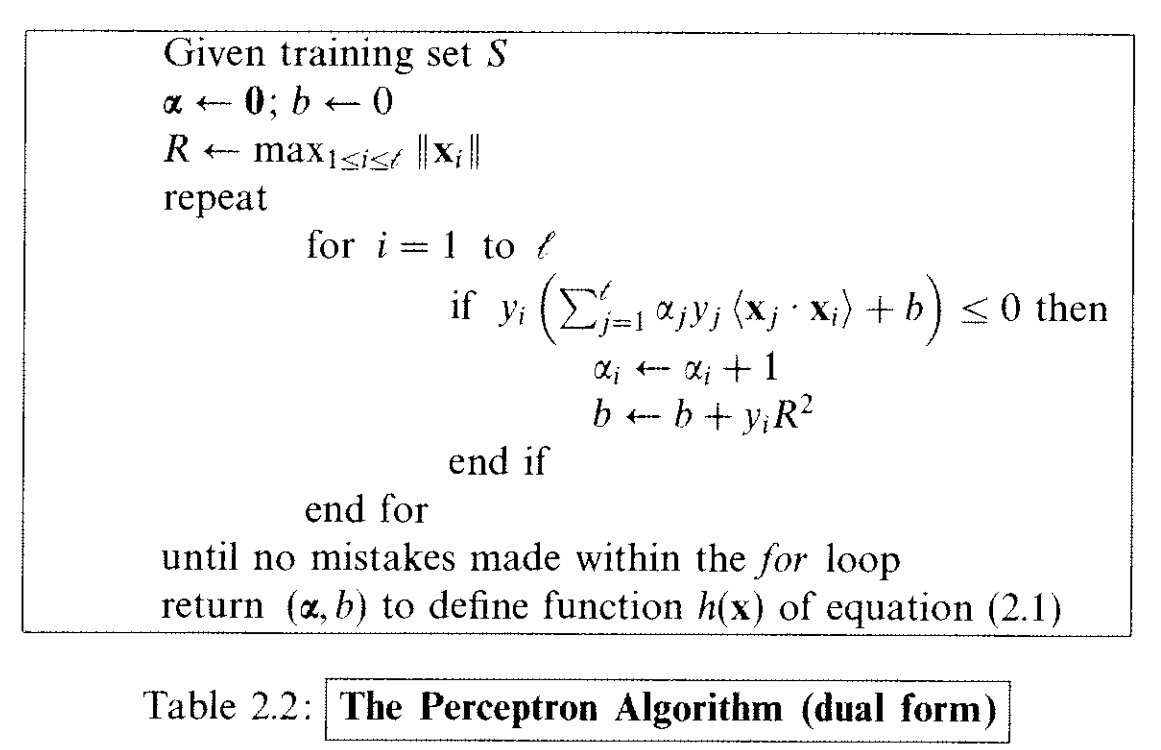
\includegraphics[width=0.7\linewidth]{pseudocodice_perceptron.png}
        \label{The Perceptron Algorithm (dual form)}
    \end{center}
    Come mostrato in (figura \ref*{The Perceptron Algorithm (dual form)}) l'algoritmo sfrutta un training set S, ovvero dati che servono al Perceptron per addestrare i parametri del classificatore: 
    \begin{itemize}
        \item $\alpha$ : 
    \end{itemize}
\end{document}